\documentclass[12pt]{article}

\newcommand\floor[1]{\lfloor#1\rfloor}
\newcommand\ceil[1]{\lceil#1\rceil}

\usepackage{amsmath}
\usepackage[super]{nth}
\usepackage[utf8]{inputenc}
\usepackage[T1]{fontenc}
\usepackage{textcomp}
\usepackage{gensymb}
\usepackage{graphicx}
\usepackage{changepage}
\usepackage{hyperref}

\pagenumbering{arabic}

\makeatletter
\newcommand*{\rom}[1]{\expandafter\@slowromancap\romannumeral #1@}
\makeatother

\begin{document}

\title{Music Generation in ArtToMusic}
\author{Rafael De Smet}

\maketitle
\tableofcontents

\section{Introduction}

In this paper I will discuss several methods to generate music with software. Analogous to the paper in graphical analysis, I will discuss methods I use in the ArtToMusic project and methods I did not use and compare them to each other. Since music is different for every person, my reasoning can be subjective at times and you may prefer other methods. 

\section{Music theory}

\subsection{Tempo and harmony}

When we listen to music, unconsciously we focus on a couple of things to process what we are hearing.

\subsubsection{Tempo}

One of these things is the tempo. A very simple way to talk about music and to distinguish between different pieces of music is to determine whether it's a fast or a slow piece. This discussion can be subjective as different people have different notions of speed. Luckily we can objectively determine the tempo of a piece, using the BPM (beats per minute).
This tells us how many quarter notes are played in one minute, or how fast/slow the quarter notes are played after each other.
\newline

In music theory there are a couple of terms to indicate certain intervals of speed, based on the BPM. For example, the term \textit{larghissimo} means that the piece of music has a BPM in the range ]0, 20], which is very slow. \textit{Moderato} means moderate, a piece that has a moderate speed usually has a BPM in the range [108, 120]. Most of the popular songs you hear on the radio are \textit{moderato}.

\subsubsection{Melody}

A second crucial part of music is the melody. All melodies of songs are based on the rules of harmony. We can formulate a couple of questions that will help us understand the purpose of harmony, e.g. which notes sound good when played together, and which don't? Which notes make up a chord?
\newline

The notion of chords is very important. A chord is a group of notes played at the same time.
There are major chords, which sound happy, and there are minor chords which sound sad or melancholic. These two types of chords are the most commonly used. There are many other types of chords such as the diminished, the sus4, add9 etc. But for this project I will stick to the two most important types and one special chord, the diminished.

\subsection{Chords and progressions}

A crucial element of music is the use of chord progressions. The most common example of this is a twelve bar blues. This type of music is characterized by a strict pattern. Every song that uses a twelve bar blues schema follows the same chord progression and thus sounds very similar and recognizable, see figure 1.

\begin{figure}[h]
\centering
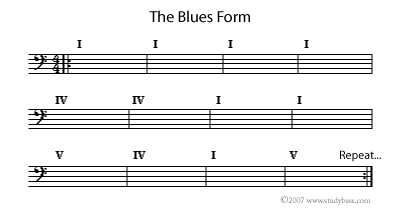
\includegraphics[scale=0.8]{img/the-blues-form}
\caption{Twelve bar blues}
\end{figure}

The roman numbers denote which chord is played, relatively to the key of the song. For example if the piece is in the key of C major, the \rom{1} denotes the first chord of the key, the C chord. The \rom{4} is the fourth chord of the key, the F major. The \rom{5} is the fifth of the key, the G major.
\newline

There are many other kinds of progressions, e.g. \rom{1}-\rom{2}-\rom{5}-\rom{1}, or any other combination. Most popular songs use multiple chord progressions, one for the verse, one for the chorus and so on. It's the concept of combining different chords in one progression that allows us to create new original pieces of music.
\newpage

\section{Music generation technologies}

In this section I will be comparing multiple music generation technologies. I will discuss libraries as well as online applications that have the same goal, creating enjoyable music based on software.

\subsection{Beads}
The Beads library, developed by Ollie Bown with the support of the university of Melbourne, is a very handy tool to generate music. Beads uses the concept of unit generators (UGs) as the core of the software. As described by Evan Merz, the author of \textit{Sonifying Processing: The Beads Tutorial} [2], a unit generator is a ``building block of the audio signal''.  One unit generator takes care of one function in the generation of music. 
\newline

A simple example of a unit generator is a guitar player's distortion pedal. The clean signal of his guitar enters the unit generator and a distorted version of the signal is produced. Beads works as a series of unit generators (or guitar pedals). You can plug one UG into another to create a chain of effects, sounds etc... 
\newline

The Beads library has many of these UGs, such as an envelope filter, a gain, a waveplayer, etc. The AudioContext is the main UG where every other UG plugs into. Without this there is no music. It doesn't create any sound by itself, it just acts as an interface to the computer's hardware. The audio comes from other UGs.
\newline

Beads has two main ways of creating audio.

\paragraph{Samples}

You can load multiple samples for later use. Once you have found the file and loaded it via the SamplePlayer, you can use it as any other UG, connect it to the Gain UG to determine the volume or apply multiple effects on it, such as pass it through an EnvelopeFilter, etc.  

\paragraph{Waves}

Another technique is to use audio waves that are generated in real time. The most simple form of audio is a sine wave that produces one tone. Beads has implemented five different kind of waves, each called a Buffer. Each Buffer stores an array of floats in the range [-1,1] that represent the function it is based on. In the following list you can see the different buffers and their functions.
\begin{itemize}
\item SINE:  based on the sine function $y(t) = A sin (\omega t + \phi)$
\item SQUARE: based on the square function $y(t) = sgn(sin(t))$
\item TRIANGLE: based on the triangle function, with range from -1 to 1 and period 2a, $y(t) = \frac{2}{a}(t - a \floor{\frac{t}{a} + \frac{1}{2}}) (-1)^{\floor{\frac{t}{a} + \frac{1}{2}}}$
\item SAW: based on the saw function $y(t) = t - \floor{t}$
\item NOISE: based on a random variable to determine each value in the buffer
\end{itemize} 

\begin{figure}[h]
\centering
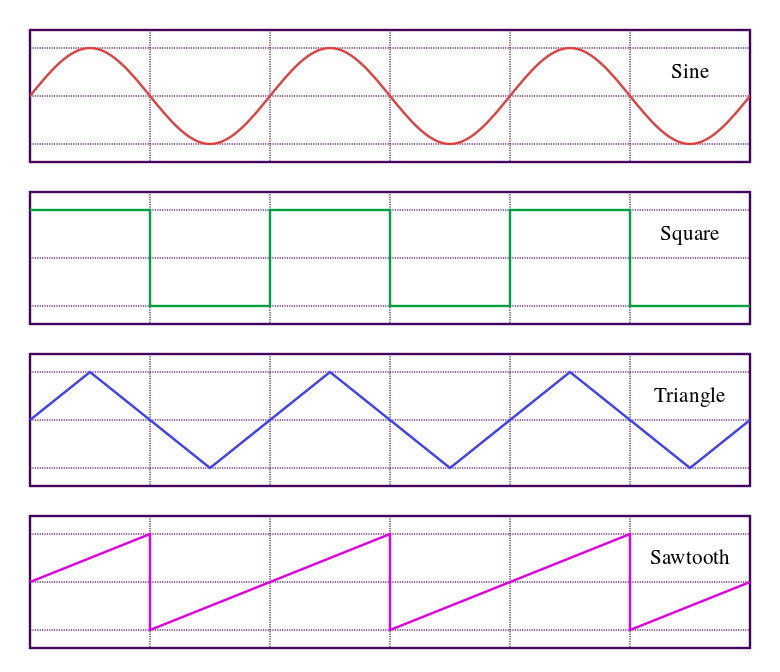
\includegraphics[scale=0.45]{img/waveForms}
\caption{Buffer functions}
\end{figure}

Every Buffer has other (mathematical) characteristics and thus sounds differently. A sine wave produces a gentle tone, while a saw wave is less enjoyable to listen to. With the Online Tone Generator, \url{http://onlinetonegenerator.com/}, we can hear the difference between the various functions.
\newline

Using the Beads library we can create our own music simply by passing the right input parameters to the different UG's to get the desired music.

\subsubsection{Examples}

The Beads project was started by Ollie Brown and has support from the Monash University in Melbourne but has since then been an open source project. When you go to the library's website [1], you can download the latest version of source code. This code contains several tutorial projects that showcase how the library works. There are eight different tutorials or lessons,  provided, increasing in complexity. It starts off easy with an explanation on how to use the AudioContext UG in code (Lesson01\_AudioContext) and ends with a complete runnable program that generates random music based on some input UGs (Lesson07\_Music).

\begin{figure}[h]
\centering
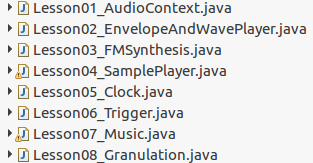
\includegraphics[scale=0.67]{img/beads_tut}
\caption{Beads tutorial projects}
\end{figure}

I will discuss the code and results of Lesson07\_Music to give the reader an idea of the capabilities of the Beads library. I provided a small application that plays the results of this lesson and other examples later in this paper. To hear the results of the Lesson 07, click on \textbf{Music Demo} in the Beads cell.

\paragraph{Code of main melody part}

This code uses a Clock UG as the basis of the generated music. A Gain and an AudioContext are there as well but these are mandatory to have in your code. The Clock is a special type of UG because it works just like a regular clock, which makes it run for ever (till you terminate the program). The Clock receives messages on-the-fly that determine what notes when to play. There are a few advantages of using a Clock as the basis. First, you can work with the concept of beats per minute (BPM). We add a new note to the Gain every beat we encounter. This note is generated from a scale which was chosen by the programmer when he wrote the code. In this case we are working with a mixolydian scale based on a random chosen pitch. From this scale we generate a random note which is then added to the Gain to be played by the Au	dioContext.

In the code you can use multiple Buffers (the type of sound wave we use to generate the frequencies heard). To generate the main melody of the song the Sine wave is used, which is the most enjoyale of all to listen to.

\paragraph{Code of bass part and rhythm} 

The code used to generate a bass part and a rhythm part is very similar to the above code. For the bass part we again can choose between multiple scales and buffers. In this case we use a pentatonic scale based on a random chosen pitch. To make it sound more simplistic and not too dominant in regards to the main melody part we use a Square wave as the Buffer. This produces slightly harsher sounds and more cut off notes than the Sine wave.

The rhythm is generated using the concept of Noise. Noise in audio is anything that's not a note, for example the noise of an old TV when the channel was of the air (what is called snow). This sound is not pleasant to hear but when we strategically play small bits of this noise it sounds like a snare drum playing a rhythm. Again, the code determines randomly when to play this noise. 

\paragraph{Sample Lesson}

The previous demo shows what Beads can do by generating music autonomously. Lesson04\_SamplePlayer is a tutorial to use the SamplePlayer UG. This loads a sample and plays it. You can again run this sample through different UGs to modify the sound as you want. To hear the results of this lesson, click on \textbf{Sample Demo} in the Beads Cell. 

\subsubsection{Conclusion}

In conclusion we can say that by using the Beads library music can be randomly generated. The benefit of this library is that you can easily integrate it in your own application and that it handles all of the communication with your system's audio device. The disadvantage of it is that it takes quite a bit of experimenting and work to fully understand how the code works and how to use it yourself.

\subsection{Wolfram Tones}

Designed by the mathematician Stephen Wolfram, WolframTones is an online application to generate music. The user can choose from multiple styles of music and the application generates a new piece of music. The way this works is based on a discovery of Stephen Wolfram himself. In the early 1980s Wolfram was researching ``one-dimensional cellular automata''. He discovered that a set of very simple rules can create a very complex situation. 
\newline

His experiments start with a row of cells, each cell black or white. The set of rules, determined before the execution, decide which colour every cell on the next line will get and so on. Figure 3 shows a possible set of rules. The top row in each box gives one of the possible combinations of colors for a cell and its immediate neighbors. The bottom row then specifies what color the center cell should be on the next step in each of these cases [1]. The rules of figure 2 can be described as follows. A particular cell will be black if either of its neighbors was black on the step before. A cell will be white if both its neighbors were white on the step before.

\begin{figure}[h]
\centering

\includegraphics[]{img/wolframRules}
\caption{Rules for automata}
\end{figure}

\begin{figure}[h]
\centering
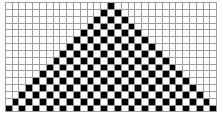
\includegraphics[]{img/wolframResult-15}
\caption{Result automata}
\end{figure}

This gives the result in figure 4. In this case the result is very well structured and organized. Wolfram discovered that there are 256 of these simple sets of rules, based on eight individual rules. Not every one of these 256 sets gives nicely structured results.

\paragraph{Music}

Wolfram used his automata to create music. Let's say we used one of the 256 sets of rules to create a result pattern. We can take a partition through this pattern of 15 cells wide. When we flip this partition on its side we can treat it as a musical score.
Figure 5 shows the partition from a resulting pattern and figure 6 shows it as a musical score.
\newline

 \begin{figure}[h]
\centering
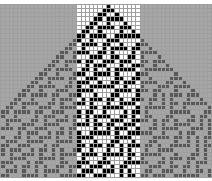
\includegraphics[]{img/wolframMusic1}
\caption{Partition through pattern}
\end{figure}

\begin{figure}[h]
\centering
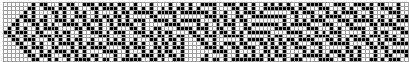
\includegraphics[]{img/wolframMusic2}
\caption{Musical score}
\end{figure}

Now we can assume that time runs across the page from left to right and every black cell represents a note played. Wolfram has developed his own programming language [4] to process these cellular automaton patterns. The music generation process is black-box.
\newline

The number of rules isn't limited by eight individual rules. We could also determine the color of the next cell by looking at his five upper row neighbors, instead of three. This gives a much bigger number of results (around 4 billion) and much more interesting results to use in the music creation. 

\subsubsection{Examples}

WolframTones is a web application [4] and therefore mostly black-box and closed-source. Every time you open the website, it generates a random piece of music on its own. There are multiple input parameters you can change to create music that fits your requirements. One of them is the music style, the site allows you to choose your own style from a wide variety of styles.

\paragraph{Algorithm Control}

Next is the Algorithm Control. Here you can choose the program to be used to generate the composition. These inputs determine the rule type and the specific rule (see above) used to generate music. You can set other parameters such as the seed and the height of the rule. The seed means what random seed you will use for any random selection that is made during the process.

\paragraph{Instrumentation}

In this section you can choose what instruments you want to hear in the piece. You can choose from 117 of the 128 MIDI instruments. The sound effects (MIDI 121 - 128) and a few other weird sounds such as a whistle are not included in the list of choices. Per instrument you can choose the role of this instrument in the song. There are 119 roles to choose from, varying from playing chords in a swing feel to playing a hip-hop inspired bass part. For every song you can select up to five instruments, each with their own individual role. This means we have in total 117*119*5 = 69615 different combinations of five instruments playing together.

To make things even more complicated you can also add a percussion part where you can choose from 111 types of percussion, ranging from a reggae beat to a jazz beat.

\paragraph{Pitch Mapping}

Every song has a central key that determines which notes are dissonant and which sound good. In this section you can choose a musical scale and a pitch where this scale is based on. WolframTones has a massive collection of scales to choose from, to be exact 404 different scales. These range from the common Western scales such as the Harmonic Major, the Blues scale etc to the more unknown ones, such as the Indian scales, the Japanese scales etc.

There are 48 different pitches you can choose to base your scale on, these range from C1 (number 24 and  a low C) to C5 (number 72, a relatively high C). Again many choices to form a unique piece of music.

\paragraph{Time Control}

The last section is the Time Control where you can determine the BPM, the notes per beat and the duration of the song. The BPM is straightforward (see above for more information about this) and ranges from 24 (very slow, \textit{larghissimo}) to 288 (very fast, even faster than \textit{prestissimo}).
The notes per beat range from 1 note per beat to 16 notes per beat, which leads to a very chaotic piece of music.
\newline

In the application I provided you can find examples of a few different combinations I tried on the website. Below is explained what choices were made for each result.

\begin{enumerate}
\item Rock/Pop style, based on rule type 31 (r=2) and rule number 3000041762. Random seed is set to 6800 and height of the score is 12. There are three instruments playing, each with another role.
\begin{itemize}
\item Electric Bass (Pick) with role: Bass - Driving
\item Guitar (Jazz) with role: Lead - Upper Part
\item Rock Organ with role: Lead - Lower Part - Legato 
\end{itemize}
A Funk 3 percussion track is also added. The scale is a Minor scale based on the F2 pitch, number 53. BPM is 116 with two notes per beat and the piece is 15 seconds long, 60 steps. Click on \textbf{Wolfram Demo 1} in the WolframTones cell of the application to hear this music.

\item R\&B style, based on rule type 7 (r=1) and rule number 168230930. Random seed is set to 123721 and height of the score is 16.
There are three instruments.
\begin{itemize}
\item Electric Bass (Finger) with role: Bass - Driving
\item Trumpet with role: Lead - Upper Part - 4x4 Loop
\item Grand Piano with role: Lead - Moving - Shorter - Legato 
\end{itemize}
A Hip Hop 1 percussion track is added. The scale is a Blues With Leading Tone scale based on the B1 pitch, number 47. BPM is 88 with 4 notes per beat and the piece is 15 seconds long, 88 steps. Click on \textbf{Wolfram Demo 2} in the WolframTones cell to hear this music.

\item Ambient style, based on rule type 1585 and rule number 338039596. Random seed is set to 10839 and height of the score is 13.
There are four instruments.
\begin{itemize}
\item Electric Piano 2 with role: Polyphonic - Length 4+
\item Electric Bass (Fretless) with role: Bass - Moving - Legato
\item Harp with role: Lead - Moving - Shorter - Medium
\item Bright Piano with role: Chords - Comp
\end{itemize}
A Jazz 1 percussion track is added. The scale is a Harmonic Minor scale based on the G\#2 pitch, number 56. BPM is 38 with 3 notes per beat and the piece is 14 seconds long, 28 steps. Click on \textbf{Wolfram Demo 3} in the WolframTones cell to hear this music.
\end{enumerate}

To show what happens when we alter only one parameter, I changed the scale, number of notes per beat and the random seed of Demo 3. To hear the version of Demo 3 with the Major Pentachord scale, click on \textbf{Wolfram Demo 3 Other Scale}. To hear the version of Demo 3 with 5 notes per beat, and again the Harmonic Minor scale, click on \textbf{Wolfram Demo 3 More NPB} (NPB is Notes Per Beat). To hear the version of Demo 3 with the random seed set to 15159, click on \textbf{Wolfram Demo 3 Other Random Seed}.

\subsubsection{Conclusion}

WolframTones is a very powerful tool to create music. It is very easy to use and understand. The big advantage of this for a user is the clear way to define the characteristics of your piece of music. WolframTones provides you with the notion of musical styles and scales, rhythm etc. When we look at Beads these concepts were not so clear when providing the input parameters. This makes WolframTones a very easy tool to use. The only disadvantage is the fact that is mosty black-box and restricted to a website, so a programmer who wants to use this technique can't download code or a library to work with himself.

\subsection{Genetic algorithms}

Another interesting case to focus on is the use of genetic algorithms to produce music, as explained in the paper by Dragan Mati\'c [2].
\newline

A genetic algorithm (GA) is based on the idea of natural selection. The execution of a genetic algorithm starts with an initial population of individuals. During the execution of the algorithm, it will try and find an optimal solution based on predetermined rules. Each individual of the population has an attribute 'fitness'. This attribute denotes the quality of each individual of the population.
\newline

The particular GA used in the paper of Dragan Mati\'c uses complete musical compositions as the individuals of the population. A composition is any combination of rhythm and notes, while the concept of good and bad music is represented in the fitness attribute. Because the notion of good and bad music is very subjective and different for each person, Mati\'c uses a reference individual (another composition) for the evaluation of the resulting composition.
\newline

We start with the initial population, containing $n$ individuals. After this, an iterative process begins. The fitness of each individual is calculated in each iteration. Based on the best individual (best fitness), we test if the stop condition is met. This stop condition can be set by the user before execution. If the algorithm decides to stop, the best individual is played.
\newline

If the algorithm continues, we remove two-thirds of the individuals in the population. Mutation operators are applied to the remaining individuals to generate new different individuals. Now the next iteration starts and we calculate the fitness of the new individuals and test if we have found a good composition.
This continues till the stop condition is met.

\paragraph{Determining the fitness}

This GA uses a function to compute the total fitness of an individual based on different criteria. Since there is an extra subjective aspect to music, the end result of the algorithm may comply to the criteria of the fitness function but still seem a bad choice (bad piece of music) to the listener. 
\newline

Equation 1 gives the total fitness of one individual. $\lambda_i$ represents the weight of the value $f_i$ to the total fitness and $n$ is the number of criteria [5].

\begin{equation}
f = \sum_{i = 1}^{n}\lambda_i f_i
\end{equation}
\\
There are a couple of ways to calculate this. You can say that for different $i$, $f_i$ may be a ratio between the number of tones out of a given tonality and the total number of tones, the ratio between the number of dissonant intervals and all intervals, the ratio between the number of appearances of some pattern in relation to the total number of notes, the density of notes, etc [2]. 
\newline

The approach of the GA in the paper of Mati\'c uses a more general approach. You calculate the fitness for each bar and the and the total fitness is the sum of those values. Now, we have a new definition for $f$.

\begin{equation}
f = \sum_{j = 1}^{k} \sum_{i = 1}^{n}\lambda_{ij} f_i
\end{equation}
\\
where $\lambda_{ij}$ is the weight of value $f_i$ in the $j^{th}$ bar, $n$ is the total number of criteria and $k$ is the total number of bars.

\paragraph{Comparison to the reference individual}

To know if the GA has chosen a good piece of music, we must compare it with the predefined reference individual. For this comparison we need a measure of similarity. This is determined based on the dissimilarity between them. To calculate the dissimilarity we use the note distance and the number and type of "good" intervals.
\newline

These intervals are predefined. See table 1 at the top of this page for a proposal of the values assigned to these intervals [2]. An interval here means two consecutive notes in a bar and their relation to each other. Are they in unison, a perfect fourth etc? Based on these values given to every note combination we can compute the fitness level of a bar of music.

\begin{figure}
\begin{tabular}{| c | c | c | c |}
\hline
\textbf{Categories of intervals} & \textbf{Intervals} & \textbf{Values Proposal} \\
\hline
Perfect Consonants & unison, perfect fourth, & 1  \\ 
& perfect fifth, octave & \\
\hline
Imperfect Consonants & minor and major thirds & 2 \\
& and sixths & \\
\hline
Seconds & minor and major seconds & 3 \\
 \hline
Sevenths & minor and major sevenths & 3 \\
\hline
Intervals greater & all intervals greater & 5 \\
than octave & than octave & \\

\hline
\end{tabular}
\end{figure}

\newpage

\subsubsection{Examples}

\subsubsection{Conclusion}

\subsection{Computoser}

Computoser is another web application that generates random music. It is a rule-based, probability-driven algorithm. This means that it composes by following a set of rules and makes decisions between several (musical) alternatives based on predefined probabilities.
\newline

Computoser gives probabilities to every type of note interval (analogous to the intervals in the GA section) and to each note length.
This means that for example a fifth (a distance of five notes in the scale) gets a probability of 25\%. This is a fairly high chance because a fifth is very commonly used in composing.
\newline

Computoser uses seven groups of rules.
\begin{enumerate}
\item Structure of the piece of music 
\item Rhythm: notes must conform to a rhythm scheme
\item Repetition: each component of the piece (a group of notes) is repeated several times for memorability 
\item Variations: slight changes are made to each component to make it more interesting
\item Dissonance and syncopation: unexpected elements in music are what makes it interesting to listen to
\item Endings: there are several predefined ways to end a piece of music
\item Effects: different kind of sounds, such as distortion, tremolo etc
\end{enumerate}

Analogous to the probabilities given to intervals, each of the rules used in the algorithm has a certain percentage that decides which rule to use.
\newline

The components of the Computoser algorithm are called manipulators. They each fill in a part of information of the score. Analogous to the Unit Generators of the Beads library, these work as a chain. Subsequent manipulators depend on previous ones. There are four main manipulators.
\newline

\begin{enumerate}
\item Part configurer: what parts are there in the piece? Is there a bass line, a piano part?
\item Scale configurer: what scale/key is the piece in? The most likely scales are the major and minor scales. Scales like the Dorian are less likely.
\item Meter configurer: what meter is the piece in? 4/4 is the most common meter, but you can have a piece in 6/8, 3/4, etc.
\item Part generator: each part has its own generator and decides for each part what notes to play.
\end{enumerate}
 
The part generator is obviously the most important one of the algorithm, because it decides what notes to play. There are three main aspects to this generator, pitch, length and variation. Again, the decisions are all based on probabilities.

\paragraph{Pitch} Apart from using the probabilities there are a few other constraints used to determine what note to play next. First, there should not be more than two subsequent unstable notes. Unstable notes are notes that are quite dissonant. Secondly, long jumps between notes (more than 7 steps/notes) require a step in the opposition direction. Thirdly, a predefined sequence of notes may be used, if they are from the circle of fifths or part of an extended chord.

\paragraph{Length} Both probabilities and some other constraints are used. The first is the measure size, all measures should have the same length. The second constraint is rhythm. Each measure is either simple (only one down-beat, e.g. 2/4) or compound (more than one down-beat, e.g. 4/4).

\paragraph{Variation} Computoser uses motifs to construct the parts. There are a few simple motifs that we use as a basis. These motifs can undergo several musical variations to create new ones. A few of these are transposition (all notes go higher or lower within the same scale), inversion (turning the melody 'upside-down'), retrograding (playing the motif backwards), etc.

\subsubsection{Examples}

\subsubsection{Conclusion}

\begin{thebibliography}{1}

\bibitem{beads} Ollie Bown (http://www.beadsproject.net/) 2008

\bibitem{beads_sonifying} Evan X. Merz {\em Sonifying Processing: The Beads Tutorial} 2011

\bibitem{wolfram} Stephen Wolfram {\em A new kind of science} 2002

\bibitem{wolframtones} http://tones.wolfram.com/

\bibitem{wolfram language} The Wolfram Language Documentation Center {\em http://reference.wolfram.com/language/guide/LanguageOverview.html}

\bibitem{genetic} Dragan Mati\'c {\em A genetic algorithm for composing music} 2010, Faculty of Natural Sciences, University of Banjaluka, Bosnia and Herzegovina

\bibitem{computoser} Bozhidar Bozhanov {\em Computoser - rule-based, probability-driven algorithmic music composition} 2014,  independent researcher

\end{thebibliography}

\end{document}